This chapter presents an analysis of the dataset used. On Section \ref{sec:dataset_desc} an overall description
and main statistics are shown. Section \ref{sec:dataset_prep} presents an early analysis of the data along with
the preprocessing steps taken. Finally section 3 makes an analytical definition of the problem
of learning urban perception from this data.


\section{Description}
\label{sec:dataset_desc}
As was mentioned previously, this work is based on the Place Pulse 2.0 dataset \cite{hidalgo_placepulse}.
PP 2.0 is a crowdsourced dataset designed for learning urban perception from street view like images.
Unlike regular datasets for supervised machine learning, that have labels for each image, Place Pulse
consists of pairwise comparisons between images, and the ground truth is a vote representing which of
the images is more representative of an attribute (ties are also possible). That structure makes
traditional classification / regression approaches inapplicable, but opens the door for
pairwise based ranking techniques, that are more suitable to urban perception since a ground truth for
how much an image represents an abstract attribute such as "safety" it's impossible to define.

The dataset consists of approximately 1.2 million pairwise comparisons of 112,000 images from 56 cities,
distributed on 6 attributes: wealthy, safety, depressing, boring, lively and beautiful, making it
the biggest available dataset for urban perception. The crowdsourcing survey was
active for 5 years and it was answered by 81,630 different users. Demographic information
about the users was not collected.

\section{Analysis and preprocessing}
\label{sec:dataset_prep}

As a first preprocessing step all noisy images are removed by using a file size threshold,
since files small in size are mostly  google api errors or unintelligible places like
dark tunnels.

It is important to note that, unlike most crowdsourced datasets, the authors of PP did not
perform a validation on the votes. 99.59\% of the image pairs that appear in the
data set have a single vote in a category (see \ref{fig:rep_hist} for details),
making it impossible to corroborate if they are reasonable by comparing the votes of multiple people.
Even though previous research indicates that answers to this surveys aren't affected by user
bias or demographics \cite{hidalgo_inequality, costa_lisbon}, the inconsistency in the votes is a
clear dataset disadvantage: 34\% of the  pairs that have more than one vote in an attribute
show inconsistencies between the votes.


\begin{figure}[ht]
	\begin{center}
	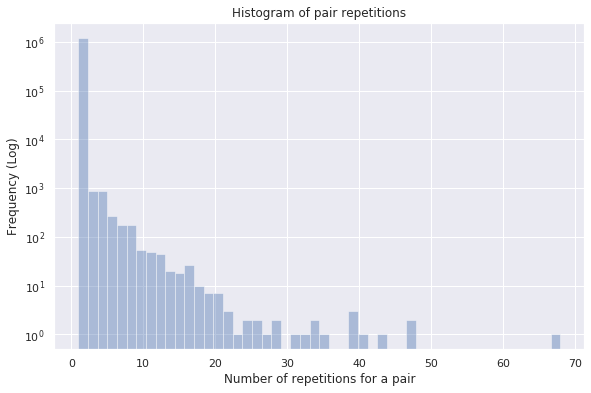
\includegraphics[width=0.8\textwidth]{./figures/rep_hist.png}
	\caption[Repetition histogram]{ Histogram for amount of repetitions for each pair of images }
	\label{fig:rep_hist}
	\end{center}
\end{figure}

For this work we completely remove all inconsistent duplicates and keep a single instance of those consistent.
After these, steps 1,207,938 votes for 111,299 images are left. See Table \ref{tab:votes}
for the exact vote distribution.

\begin{table}[H]
	\begin{center}
	\caption[Votes Distribution]{ Vote distribution after preprocessing.}
	\begin{tabular}{ll}
		\hline
		\textbf{Attribute} & \textbf{\# of votes} \\ \hline
		Wealthy            & 150,370               \\
		Safety             & 364,130               \\
		Depressing         & 130,781               \\
		Boring             & 125,744               \\
		Lively             & 263,123               \\
		Beautiful          & 173,790               \\ \hline
		Total              & 1,207,938            \\
	\end{tabular}
	\label{tab:votes}
	\end{center}
\end{table}

Users of the survey had the possibility of voting that a pair is tied for an attribute,
meaning that they didn't perceive any significant difference. Previous works usually
discard this data and don't use it for learning, focusing only on the votes where a preference was
chosen \cite{hidalgo_placepulse,zhang_measuring,tamara_judgments}. After preprocessing 15.3\% of the
votes are ties, which means a significant amount of information is lost by disregarding them.
Due to that we decided to add additional rules to the learning problem in order to be able to use
these votes for learning. Details are shown on the following chapter.